\begin{abox}
	Assignment-S05\\
	\vspace{0.5cm}
Magnetic Vector Potential, Magnetic Dipole
	\end{abox}
\begin{enumerate}
	\item $\left. \right. $
	\begin{answer}
			(a) $\overrightarrow{\mathrm{A}}$ point in the same direction as $I$ and is a function of $r$ (the distance from the wire).
		\begin{align*}
		\text{In cylindrical coordinates }\vec{A}&=A(r) \hat{z}\text{ and }\vec{B}=\vec{\nabla} \times \vec{A}=-\frac{\partial A}{\partial r} \hat{\phi}=\frac{\mu_{0} I}{2 \pi r} \hat{\phi}.\\
		\Rightarrow \frac{\partial A}{\partial r}&=-\frac{\mu_{0} I}{2 \pi r} \Rightarrow \vec{A}(r)=-\frac{\mu_{0} I}{2 \pi} \ln \left(\frac{r}{a}\right) \hat{z} \text{(Constant $a$ is arbitrary)}\\
		\text{Verify that }\vec{\nabla} \cdot \vec{A}&=0\text{ and }\vec{\nabla} \times \vec{A}=\vec{B}\\
		\Rightarrow \vec{A}(r=R)&=-\frac{\mu_{0} I}{2 \pi} \ln \left(\frac{R}{2 R}\right) \hat{z}=\frac{\mu_{0} I}{2 \pi} \ln 2 \hat{z}\\
	\text{	(b) }\oint \vec{B} \cdot d \vec{l}&=B \cdot 2 \pi r=\mu_{0} I_{e n c}=\mu_{0} J \pi r^{2}=\frac{\mu_{0} I}{\pi R^{2}} \pi r^{2}=\frac{\mu_{0} I r^{2}}{R^{2}} \Rightarrow \vec{B}=\frac{\mu_{0}}{2 \pi} \frac{I r}{R^{2}} \hat{\phi}\\
		\vec{B}&=\vec{\nabla} \times \vec{A}=-\frac{\partial A_{z}}{\partial r} \hat{\phi} \Rightarrow \frac{\partial A}{\partial r}=-\frac{\mu_{0} I}{2 \pi} \frac{I r}{R^{2}} \Rightarrow \vec{A}=-\frac{\mu_{0} I}{4 \pi R^{2}}\left(r^{2}-b^{2}\right) \hat{z}\\
	\text{	where $b$ is }&\text{arbitrary constant.}\\
		\Rightarrow \vec{A}\left(r=\frac{R}{2}\right)&=-\frac{\mu_{0} I}{4 \pi R^{2}}\left(\frac{R^{2}}{4}-\frac{R^{2}}{16}\right) \hat{z}=-\frac{\mu_{0} I}{4 \pi R^{2}}\left(\frac{R^{2}}{4}-\frac{R^{2}}{16}\right) \hat{z}=-\frac{\mu_{0} I}{4 \pi R^{2}}\left(\frac{3}{16}\right) \hat{z}
		\end{align*}
	\end{answer}
	\item  $\left. \right. $
	\begin{answer}$\left. \right. $
		\begin{figure}[H]
			\centering
			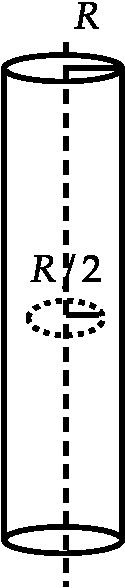
\includegraphics[height=4.5cm,width=1.2cm]{Assi-S26}
		\end{figure}
		\begin{align*}
		\text{(a) Surface current }\vec{K}&=\sigma \vec{v} \Rightarrow \vec{K}=\sigma R \omega \hat{\phi}\text{, thus }\vec{A}=A_{\phi} \hat{\phi}\\
	\text{	Magnetic field inside is}&\\
		\oint \vec{B} \cdot d \vec{l}&=\mu_{0} I_{\text {enc }} \Rightarrow B l=\mu_{0} K l \Rightarrow B=\mu_{0} K \Rightarrow \vec{B}=\mu_{0} \sigma R \omega \hat{z} \\
		\text { Since } \vec{B}&=\vec{\nabla} \times \vec{A} \Rightarrow \oint_{\text {line }} \vec{A} \cdot d \vec{l}=\int_{S} \vec{B} \cdot d \vec{a} \\
		\Rightarrow|\vec{A}| \times 2 \pi(R / 2)&=\mu_{0} \sigma R \omega \times \pi(R / 2)^{2} \Rightarrow \vec{A}=\frac{1}{4} \mu_{0} \sigma \omega R^{2} \hat{\phi}\\
		\text{(b) Since }\vec{B}&=\vec{\nabla} \times \vec{A} \Rightarrow \oint_{\text {line }} \vec{A}.\\
		\text { (b) Since } \vec{B}&=\vec{\nabla} \times \vec{A} \Rightarrow \oint_{\text {line }} \vec{A} \cdot d \vec{l}=\int_{S} \vec{B} \cdot d \vec{a} \\
		\Rightarrow|\vec{A}| \times 2 \pi(2 R)&=\mu_{0} \sigma R \omega \times \pi(R)^{2} \\
		\Rightarrow \vec{A}&=\frac{1}{4} \mu_{0} \sigma \omega R^{2} \hat{\phi}
		\end{align*}
			\begin{figure}[H]
			\centering
			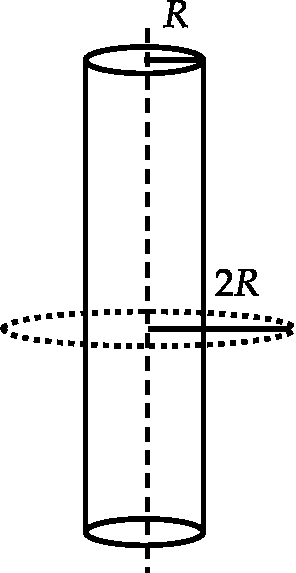
\includegraphics[height=4.5cm,width=2.5cm]{Assi-S27}
		\end{figure}
	\end{answer}
	\item $\left. \right. $
	\begin{answer}
		\begin{align*}
		\oint \vec{A} \cdot \overrightarrow{d l}&=\int_{S}(\vec{\nabla} \times \vec{A}) \cdot d \vec{a}=\int_{S} \vec{B} \cdot d \vec{a}\\&=B A \cos 60^{0}=1.2 \times\left(\frac{1}{\sqrt{2}}\right)^{2} \times \frac{1}{2}=0.30 T . m^{2}
		\end{align*}
	\end{answer}
	\item $\left. \right. $
	\begin{answer}
		\begin{align*}
		\vec{m}&=m \hat{z} \quad\text{ and }\quad \vec{B}=\vec{\nabla} \times \vec{A}=\frac{m}{r^{3}}(2 \cos \theta \hat{r}+\sin \theta \hat{\theta})=\frac{1}{r^{3}}[3(\vec{m} \cdot \hat{r}) \hat{r}-\vec{m}]\\
		\vec{B}&=\frac{1}{r^{3}}\left[3 m \hat{z} \cdot\left(\frac{x \hat{x}+y \hat{y}+z \hat{z}}{r}\right) \frac{\vec{r}}{r}-m \hat{z}\right]=\frac{1}{r^{3}}\left[\frac{3 m z}{r}\left(\frac{x \hat{x}+y \hat{y}+z \hat{z}}{r}\right)-m \hat{z}\right]\\
	\text{	(a) }B_{x}&=\frac{3 m x z}{r^{5}}\qquad
	\text{	(b) }B_{y}=\frac{3 m y z}{r^{5}}\qquad
	\text{	(c) }B_{z}=\frac{m}{r^{3}}\left(\frac{3 z^{2}}{r^{2}}-1\right)
		\end{align*}
	\end{answer}
	\item $\left. \right. $
	\begin{answer}
		 Magnetic dipole moment associated with a square shaped loop (let side is $a$ ) carrying a steady current $I$ is $m=I a^{2}$.\\
		Magnetic dipole moment associated with a circular shaped loop (let radius is $r$ ) carrying a steady current $I$ is $m^{\prime}=I \pi r^{2}$.
		\begin{align*}
	\text{	Here }4 a&=2 \pi r \Rightarrow r=\frac{2 a}{\pi} \Rightarrow m^{\prime}=I \pi r^{2}=I \pi\left(\frac{2 a}{\pi}\right)^{2}=\frac{4 I a^{2}}{\pi}=\frac{4 m}{\pi}\\
		\Rightarrow m^{\prime}&=\frac{4 m}{\pi}=\frac{4 \times 1}{\pi} \mathrm{Am}^{2}=1.27 \mathrm{Am}^{2}
		\end{align*}
	\end{answer}
	\item $\left. \right. $
	\begin{answer}
		\begin{align*}
	\text{ Magnetic moment }m&=I A=\frac{2 B R}{\mu_{0}} \times \pi R^{2}=\frac{2 \pi B R^{3}}{\mu_{0}} \quad \because B=\frac{\mu_{0} I}{2 R}\\
		\Rightarrow m&=\frac{2 \pi \times 2 \times 10^{-6} \times\left(10^{-1}\right)^{3}}{4 \pi \times 10^{-7}}=1 \times 10^{-2} \mathrm{~A} . \mathrm{m}^{2}=0.01 \mathrm{~A} . \mathrm{m}^{2}
		\end{align*}
	\end{answer}
	\item $\left. \right. $
	\begin{answer}
		\begin{align*}
		r_{n}&=n^{2} a_{0} \Rightarrow 2.04=n^{2} \times 0.51 \Rightarrow n=2\\
		\mu&=I A=\frac{e v_{n}}{2 \pi r_{n}} \times \pi r_{n}^{2}=\frac{e v_{n} r_{n}}{2}=\frac{e r_{n}}{2} \frac{n \hbar}{m r_{n}}=\frac{n e \hbar}{2 m}=\frac{n e h}{4 \pi m} \quad\\ \because m v_{n} r_{n}&=n \hbar \Rightarrow v_{n}=\frac{n \hbar}{m r_{n}} \\
		\Rightarrow \mu&=\frac{n e h}{4 \pi m}=\frac{2 \times 1.6 \times 10^{-19} \times 6.6 \times 10^{-34}}{4 \times 3.14 \times 9.1 \times 10^{-31}}=\frac{21.12 \times 10^{-43}}{114.3 \times^{-31}}\\&=\frac{211.2 \times 10^{-43}}{114.3 \times^{-30}}=1.85 \times^{-13} \text { A.m }^{2}
		\end{align*}
	\end{answer}
	\item $\left. \right. $
	\begin{answer}$\left. \right. $
			\begin{figure}[H]
			\centering
			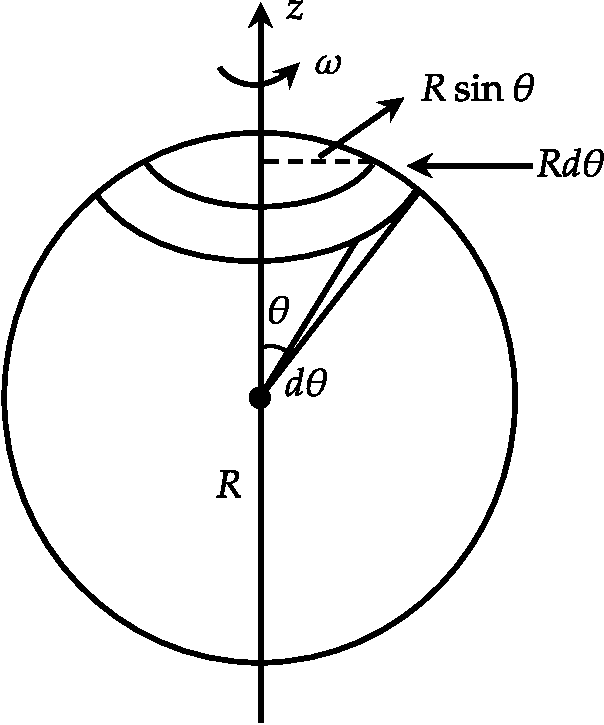
\includegraphics[height=6cm,width=5cm]{Assi-S28}
		\end{figure}
			The total charge on the shaded ring is
		\begin{align*}
		d q&=\sigma(2 \pi R \sin \theta) R d \theta\\
		\text{Time for one revolution is }d t&=\frac{2 \pi}{\omega}\\
		\Rightarrow\text{ Current in the ring }I&=\frac{d q}{d t}=\sigma \omega R^{2} \sin \theta d \theta\\
	\text{	Area of the ring }&=\pi(\mathrm{R} \sin \theta)^{2},\text{ so the magnetic moment of the ring is}\\
		d m&=\left(\sigma \omega R^{2} \sin \theta d \theta\right) \times \pi R^{2} \sin ^{2} \theta \\
		m&=\sigma \omega R^{4} \int_{0}^{\pi} \sin ^{3} \theta d \theta=\frac{4}{3} \pi \times \sigma \omega R^{4} \Rightarrow \vec{m}=\frac{4 \pi}{3} \sigma \omega R^{4} \hat{z}\\
		\Rightarrow|\vec{m}|&=\frac{4 \pi}{3} \sigma \omega R^{4}=\frac{4 \pi}{3} \times 10 \times 10^{-6} \times 70 \times\left(50 \times 10^{-3}\right)^{4}\\&=\frac{4 \pi}{3} \times 7 \times 10^{-4} \times\left(625 \times 10^{-8}\right)\\
		\Rightarrow|\vec{m}|&=18316.7 \times 10^{-12} \mathrm{Am}^{2}=0.018 \times 10^{-6} \mathrm{Am}^{2}=0.018 \mu \mathrm{Am}^{2}
		\end{align*}
	\end{answer}
	\item $\left. \right. $
	\begin{answer}	$\left. \right. $
		\begin{figure}[H]
			\centering
			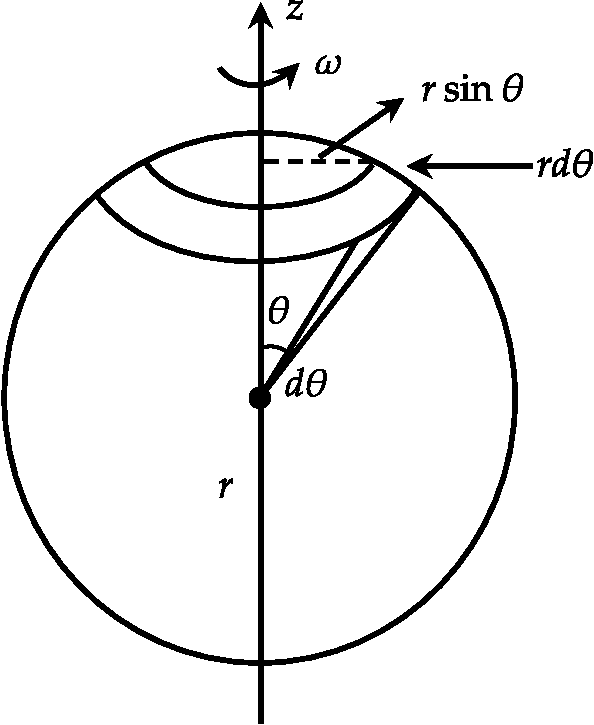
\includegraphics[height=6cm,width=5cm]{Assi-S29}
		\end{figure}
		 The magnetic moment must clearly be along the axis of rotation. Consider a volume element $d \tau$. It contains charge $\frac{q}{4 \pi / 3 R^{3}} d \tau$. The rotation of the sphere causes this charge to revolve around the axis and constitute a current:
		\begin{align*}
		&\frac{q}{4 \pi / 3 R^{3}} d \tau \times \frac{\omega}{2 \pi}\\
	\text{	Its magnetic }&\text{moment will be}\\
		&\frac{q}{4 \pi / 3 R^{3}} d \tau \times \frac{\omega}{2 \pi} \times \pi(r \sin \theta)^{2}\\
	\text{	So total magnetic }&\text{moment is}\\
		m&=\int_{0}^{R} \int_{0}^{\pi} \int_{0}^{2 \pi} \frac{q}{4 \pi / 3 R^{3}}\left(r^{2} \sin \theta d r d \theta d \phi\right) \times \frac{\omega}{2 \pi} \times \pi(r \sin \theta)^{2}\\
		\Rightarrow m&=\frac{q}{4 \pi / 3 R^{3}} \times \frac{R^{5}}{5} \times 2 \pi \times \frac{\omega}{2} \times \int_{0}^{\pi} \sin ^{3} \theta d \theta \Rightarrow m\\&=\frac{q}{4 \pi / 3 R^{3}} \times \frac{R^{5}}{5} \times 2 \pi \times \frac{\omega}{2} \times \frac{4}{3}=\frac{1}{5} q R^{2} \omega
		\end{align*}
	\end{answer}
	\item $\left. \right. $
	\begin{answer}$\left. \right. $
		\begin{figure}[H]
			\centering
			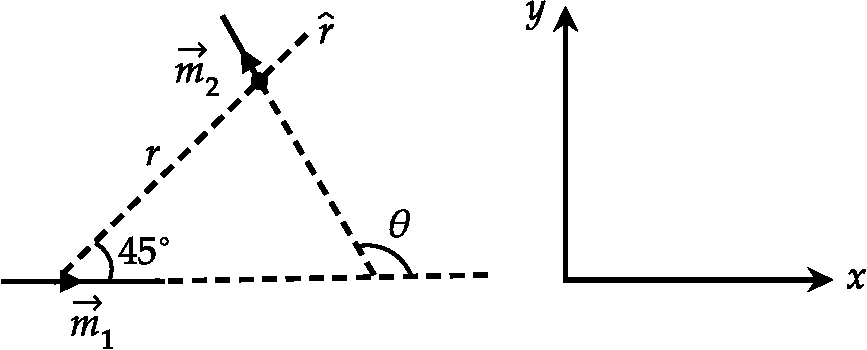
\includegraphics[height=2.8cm,width=6.7cm]{Assi-S30}
		\end{figure}
		\begin{align*}
		U&=\frac{\mu_{0}}{4 \pi r^{3}}\left[\vec{m}_{1} \cdot \vec{m}_{2}-3\left(\vec{m}_{1} \cdot \hat{r}\right)\left(\vec{m}_{2} \cdot \hat{r}\right)\right]\\
		\Rightarrow U&=\frac{\mu_{0} m_{1} m_{2}}{4 \pi r^{3}}\left[\cos \theta-3 \cos 45^{0} \cos \left(\theta-45^{\circ}\right)\right]\\
		\text{For stable}&\text{ position energy is minimum i.e.}\\
		\frac{\partial U}{\partial \theta}&=0 \Rightarrow \frac{\mu_{0} m_{1} m_{2}}{4 \pi r^{3}}\left[\sin \theta+\frac{3}{\sqrt{2}} \sin \left(\theta-45^{\circ}\right)\right]=0 \\
		\Rightarrow \sin \theta&=\frac{3}{\sqrt{2}}\left(\frac{\sin \theta}{\sqrt{2}}-\frac{\cos \theta}{\sqrt{2}}\right) \\
		\Rightarrow \tan \theta&=3 \Rightarrow \sin \theta=\frac{3}{\sqrt{10}}
		\end{align*}
	\end{answer}
	
	
	
	
	
	
	
	
	
	
	
	
	
\end{enumerate}
	
	
	
	
	
	
	
	

	
	
	
	
	